\begin{listing}[H]
  \caption{The source code for \emph{2recognizer.rb}.}
  \label{lst: source code of 2recognizer}
  \inputminted[rulecolor=gray(x11gray),linenos,frame=lines,framesep=5mm]{ruby}{code/2recognizer.rb}
\end{listing}
\addcontentssubsection{\textbf{Listing \ref{lst: source code of 2recognizer}} Source code for 2recognizer.rb} % manually adds this listing to table of contents
\begin{figure}[H] % shows screenshot output of code
  \centering
  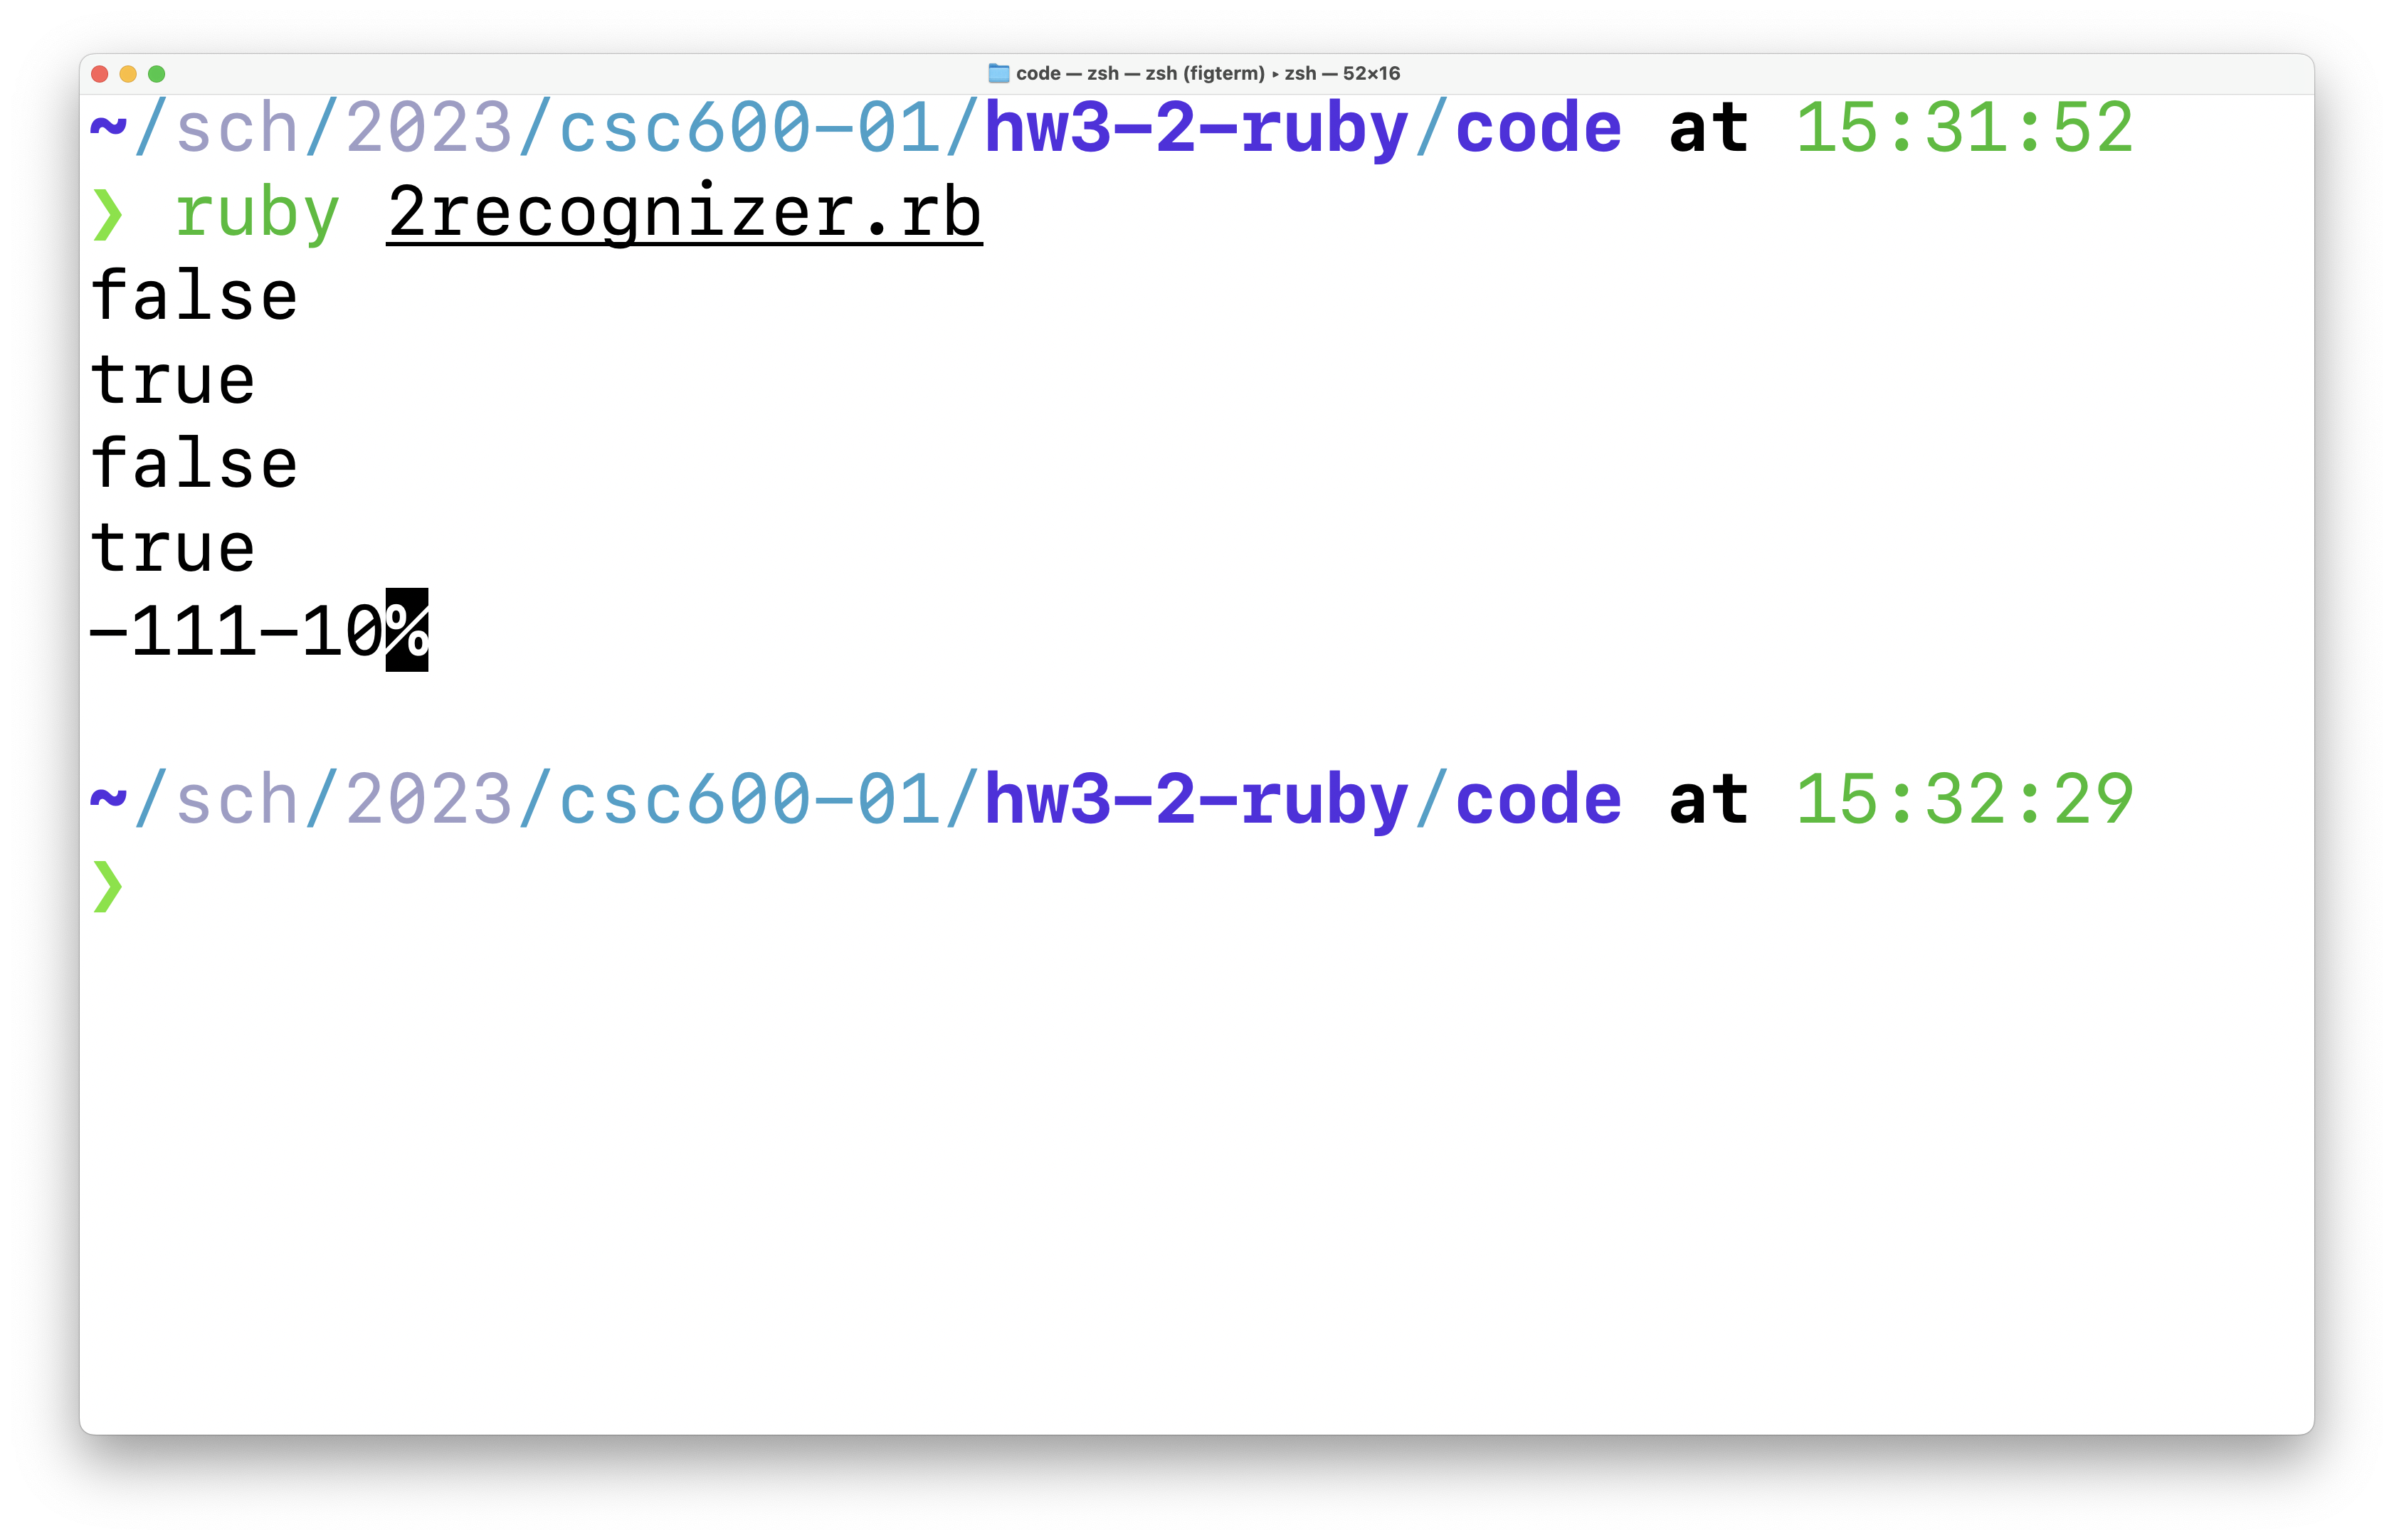
\includegraphics[height=.4\linewidth]{2recognizer.PNG}
  \setlength{\captionmargin}{0pt}
  \caption{Screenshot output of executing \emph{2recognizer.rb}}
  \label{fig:2recognizer.png}
\end{figure}
\addcontentssubsection{\textbf{Figure \ref{fig:2recognizer.png}} Screenshot output of executing \emph{2recognizer.rb}} % manually adds this listing to table of contents
